\chapter{Requirements} \label{ch:req}
This chapter will contain the requirements for the system and a test specification which will describe how to test for the requirements.

\section{Requirement specification}
\begin{table}[ht!]
  \centering
  \begin{tabular}{l l c c p{4cm} p{2.5cm}}
  \toprule
  \textbf{No.} & \textbf{Parameter} & \textbf{Value} & \textbf{Unit} & \textbf{Additional Information} & \textbf{Source} \\
  \midrule
  1 & Frame rate & $\geq 10$ & fps & & Section \vref{sec:intromotiv} \\
  \midrule
  2 & Disparity precision & $\leq 2$ & mm & $\bullet$ Either directly or using subpixel refinement & Section \vref{sec:intromotiv}\\
  \midrule
  3 & Depth range & 0.5-1.5 & m & & Section \vref{sec:intromotiv} \\
  \midrule
  4 & Camera resolution & 2592$\times$1944 & pixels & & Section \vref{sec:disppre} \\
  \midrule
  5 & Focal length & $\geq 10$ & mm & & Section \vref{sec:disppre} \\
  \midrule
  6 & Pixel size & 0.0022 & \si{\micro\meter} & & Section \vref{sec:disppre} \\  
%  \midrule
%  7 & \multicolumn{5}{p{11cm}}{The algorithm should provide a better result than a standard normalised cross correlation algorithm} \\
  \toprule
  \multicolumn{6}{l}{\textbf{General requirements}}\\
  \multicolumn{6}{l}{$\bullet$ For a camera \textit{Imaging Source DMK 72BUC02} or similar camera should be used}\\
  \bottomrule
  \end{tabular}
\end{table}
\section{Test specification}
This section will describe how to test to ensure requirements are fulfilled. \\
%\todo{Regner med at lave en test hvor jeg med min egen python simulering trækker dataen ud lige før hvor dataen skal bruges i det jeg har fået lavet et hardware design af. så vil jeg samligne med middlebury test sets}

%\todo{skriv hvordan jeg vil teste de forskellige krav}

%\todo{beskrive middlebury test sets her? Nej beskriv dem i appendix}



Requirement 1: frame rate can be tested by running the finalized implementation and measure the run time which then should be $\leq $. \\

For requirement 2: disparity precision HSA system produced a test object which has small depth increases. Figure \vref{fig:3dpretest} shows a 3D model of this test object. This model was 3D printed in case a working prototype of the prototype was available for testing. The steps closest to the bottom right of the figure increase by 1 mm for each step. The next line increase by 2 mm for each step. This continues and the last line of steps increases by 5 mm for each step. The small shapes in the middle of each step have a depth difference of 0.5 mm and alternately protrudes from or recesses into the steps. This object can be used to test where the precision of a stereo setup and algorithm is between 0.5 and 5 mm depending on which lines of step can be seen. \\

\begin{figure}[ht!]
  \centering
  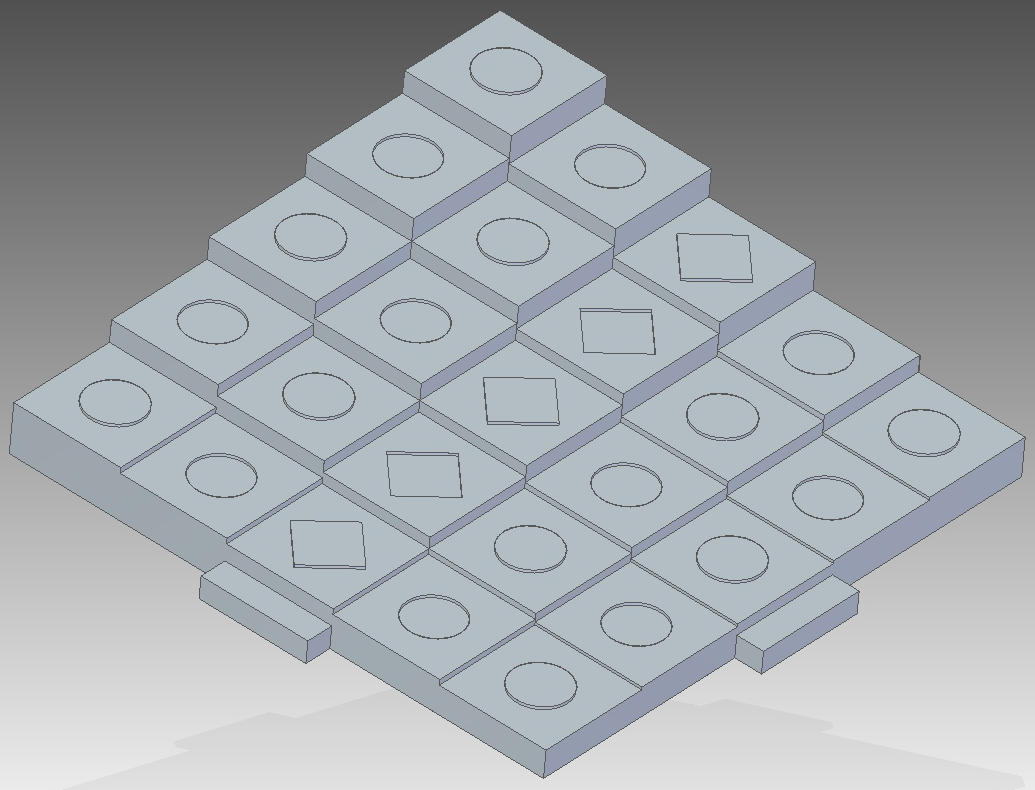
\includegraphics[width=0.5\textwidth]{figures/3dprecisiontest}
  \caption{3D model of test object for depth precision}
  \label{fig:3dpretest}
\end{figure}
The middlebury test set don't contain images where specific areas contain depth increments of 2 mm and therefore these images can't be used for testing this requirement and we are forced to rely on the calculations from section \vref{sec:disppre}. \\

Requirement 3: depth range can only be correctly tested for if a working prototype is developed.

Requirement 4: camera resolution, requirement 5: focal length and requirement 6: pixel size are fulfilled by choosing the correct camera hardware but are essential to be fulfilled for requirement 2 to be fulfilled.

Chapter \vref{ch:acctest} will perform the available tests.

